\chapter{BAYESIAN ESTIMATION OF SUBSET THRESHOLD AUTOREGRESSIVE MODELS FOR SHORT-TERM FORECASTING OF TRAFFIC OCCUPANCY}
\label{chap:traffic}
%%%%%%%%%%%%%%%%%%%%%%%%%%%%%%%%%%%%%%%%%%%%%%%%%%%%%%%%%%%%%%%%%%%%%%%
\section{Introduction}
Rising populations in major cities add stress to advanced traffic management systems (ATMS) tasked with monitoring real-time traffic variables to proactively reduce congestion. Ever since \cite{Ahmed1979} used basic ARIMA strategies to model freeway traffic networks in large US cities -- Los Angeles, Minneapolis, and Detroit -- significant research has accumulated to appropriately utilize the massive amount of data obtained in transportation networks. The global concern has manifested through independent research in major cities in places such as the United Kingdom \citep{Queen2009,Dunne2012}, Greece \citep{Stathopoulos2003, Kamarianakis2012,Theofilatos2017}, Italy \citep{Annunziato2013,Moretti2015}, China \citep{Shang2006,Jun2007,Min2010}, and Ethiopia \citep{Hellendoorn2011}. Technological advances over this time period have not only improved the gathering of the data but also in the quick distribution of pertinent information to drivers. The speed and accuracy between the detection to the correction rely on efficient modeling and accurate short-term forecasting of important traffic characteristics.

Three traffic variables have been used to quantify traffic congestion per unit of time: flow (volume per time), speed (distance per time), and occupancy (percent of time occupied) \cite{Hall1992}. \cite{Smith1997} provide insight into the state of traffic modeling 20 years ago while \cite{Vlahogianni2014} do an excellent job summarizing recent advancements in short-term traffic forecasting by posing 10 interesting challenges for future researchers. The scarcity of forecast procedures for traffic occupancy may stem from the instability acknowledged in \cite{Levin1980}. Traffic occupancy, the percent of time a detection zone is occupied, has been described as ``quality assessment measure'' as it quantifies how well traffic is moving through a network \citep{Klein1996}.  We comprehensively present univariate approaches for modeling traffic occupancy with the aim of evaluating forecasts at multiple horizons. Section \ref{sec:trafficdata}  presents a challenging traffic dataset from a major arterial in Athens, Greece, used for empirical study.

Traffic occupancy has been used to help forecast other traffic characteristics \citep{Hazelton2004}.  In regards to modeling traffic occupancy, most researchers adapt similar methods seen for traffic flow and speed \citep{Kamarianakis2010}. Like other traffic variables, occupancy exhibits abrupt changes in mean, temporal dynamics, and volatility as traffic fluctuates between free flow and congested states. Realizations of recent traffic occupancy can assist in the characterization of these states. In Section \ref{sec:trafficmodels}, we recommend the nonlinear threshold autoregressive (TAR) process to model and forecast traffic occupancy. The parametric TAR structure, first discussed in \cite{Tong1990}, is a conditional autoregressive (AR) model dependent on states governed by traffic occupancy . The model is highly interpretable making it appealing to practitioners. For easy application, TAR models for each location are defined to be day-specific and horizon-specific. Also, we present a baseline periodic linear regression model that adequately captures the seasonality exhibited in traffic data.

\cite{Ghosh2007} provide a case for the movement from classical inference to Bayesian inference in traffic models. Joint contributions from \cite{Broemeling1992,Geweke1993,Chen1995} formed the foundation of Bayesian TAR modeling. \cite{Campbell2004} applied reversible jump Markov chain Monte Carlo to select regime-specific AR orders. Subset selection of TAR via stochastic search variable selection \citep{George1993} was conducted by \citet{So2003,Chen2011}. For all the aforementioned approaches, the number of regimes must be known or assumed. In illustration, simulation, and application, TAR models are often restricted to have at most three regimes. 

\cite{Chan2015} transformed the nonlinear TAR model into a high dimensional linear regression. Multi-step procedures seek sparse solutions to identify the regimes and perform parameter estimation \citep{Chan2015,Chan2017}. The fully Bayesian approach of \cite{Pan2017} operates similarly by utilizing a sequence of binary inclusion variables to identify change points and select regimes. The fully saturated TAR model defined Section \ref{sec:trafficmodels} follows from \cite{Chan2015} with some slight modifications. 

Section \ref{sec:trafficest} proposes a fully Bayesian three step  procedure that automates selecting the regimes and sparse subset AR estimation within regimes. First, a fully saturated TAR model is estimated using Bayesian regularization implemented through a modified horseshoe prior \citep{Carvalho2009,Carvalho2010,Bhadra2016}. Next, the Kullback-Leibler (KL) divergence \citep{Kullback1951} combined with a forward selection algorithm identifies the regimes through comparing posterior predictive distributions of the linear AR model to multiple regime TAR models. Finally, given a restricted set of regimes, the same procedure is repeated to select the relevant dynamics within each of the regimes. The result is a parsimonious TAR model with a posterior predictive distribution close in KL distance to the posterior predictive distribution from the full model.

\begin{center}
NEED MORE
\end{center}






%%%%%%%%%%%%%%%%%%%%%%%%%%%%%%%%%%%%%%%%%%%%%%%%%%%%%%%%%%%%%%%%%%%%%%%
\section{Data}
\label{sec:trafficdata}

Real-time traffic data are obtained from the major Athen's arterial, Alexandras Avenue, along the westbound direction. Every 90 seconds in April 2000, traffic occupancy is captured from seven loop detectors abbreviated $L \in \{A,B,C,D,E,F,G\}$. The National Technical University of Athens is credited for the gathering of this data. The 2013 Traffic Research Board's (TRB) Annual Meeting Workshop used a larger ecompassing dataset in their TRANSportation Data FORecasting Competition (TRANSFOR). This competition was organized by the Aritificial Intelligence and Advanced Computing Applications Committee.  Many of the inherent characteristics in this dataset make short-term forecasting quite challenging. The winning methodology applied adaptive lasso to high-dimensional nonlinear space-time models \citep{Kamarianakis2012}. Figure \ref{fig:trafficdatamap} was created using Google Maps to provide a visual depiction of this small network with arrows representing direction of traffic flow. Loop detectors $A$, $B$, $C$, and $D$ measure traffic occupancy in the westbound direction, and detectors $E$, $F$, and $G$, in the eastbound direction.

\begin{figure}[htbp]
\caption{Locations of Loop Detectors Along Alexandras Ave. in Athens, Greece: Arrows Indicate Direction of Traffic Flow}
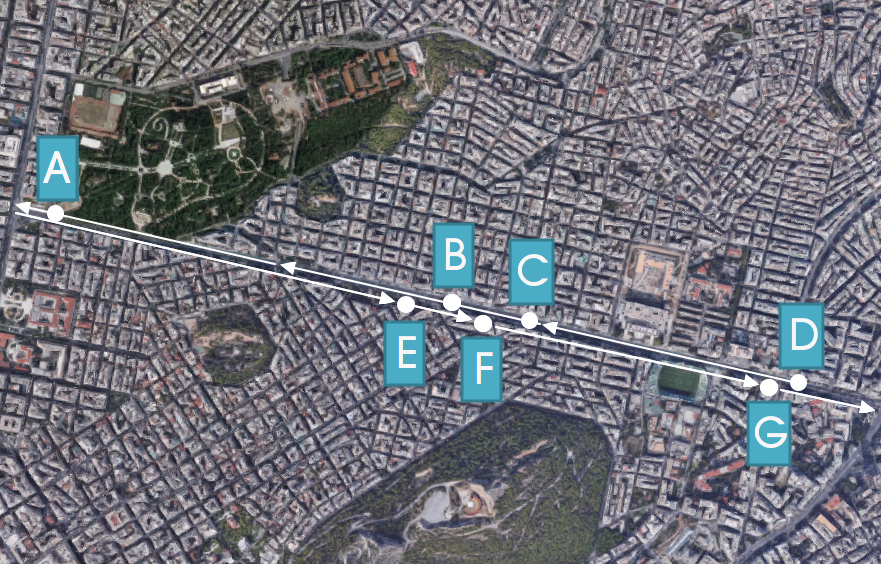
\includegraphics[width=\textwidth]{TrafficMap2}
\label{fig:trafficdatamap}
\end{figure}

Analyzing the raw traffic occupancy from an urban network measured on the 90s interval becomes problematic due to the large amount of noise seen at high resolutions \citep{Vlahogianni2014}. Temporal aggregation to larger intervals i.e. 15 min has been practiced over the years as a smoothing technique prior to modeling. Not only does this practice make short-term forecasting irrelevant with today's technology but diminishes useful long memory, nonlinear, and heteroskedastic dynamics in the underlying signal \cite{Vlahogianni2011}.Rather than modeling across different levels of temporal aggregation, as seen in \cite{Shang2006}, we average to 3 minute intervals resulting in 480 daily time points per location. 

Define random variable $O_{L,t}$ as the traffic occupancy for location $L$ at time $t$ and $o_{L,t}$ represents a known realization. As common practice, we ignore traffic occupancy data on weekends. Cyclical human behavior patterns throughout the work week lead to weekly seasonal traffic patterns. Data during April 2000 covers four complete weeks. The first three weeks are used to fit TAR models, and the last week is designated for forecasting evaluation. Time series plots of $\{o_{L,t}\}$ are found in Figure \ref{fig:OrigPlotTrafficOcc} organized by location.

\begin{figure}[htbp]
\caption{Raw Traffic Occupancy for All Locations Measured on 3-Minute Interval: Shaded Region Indicates the Forecasting Period}
\includegraphics[width=\textwidth]{rawplots}
\label{fig:OrigPlotTrafficOcc}
\end{figure}







%%%%%%%%%%%%%%%%%%%%%%%%%%%%%%%%%%%%%%%%%%%%%%%%%%%%%%%%%%%%%
\section{Threshold Autoregressive Model}
\label{sec:trafficmodels}

\subsection{General Modeling Information}
For each location $L\in \{A,B,C,D,E,F,G\}$, day of the week $D\in\{M,T,W,Th,F\}$, and horizon $h \in \{1,3,5\}$ , we build $(L,D,h)$-specific TAR models to obtain forecast $\widehat{O}_{L,t}=E[O_{L,t}|\mathcal{I}_t]$ where $\mathcal{I}_t=\{o_{L,k}\}_{k=t-h}^{t-h-P+1}$. Chosen horizons correspond to 3 min, 9 min, and 15 min ahead forecasts. The weekly periodicity of traffic occupancy modeled in \cite{Williams1999,Ghosh2007,Kamarianakis2010} and visually seen in Figure \ref{fig:OrigPlotTrafficOcc} defends $D$-specific modeling. The purpose of $h$-specific models is to ensure multi-step forecasting is user-friendly and computationally efficient for practitioners. 

The order parameter $P\in\mathbb{N}$ represents the maximum short-term lag relevant for forecasting and should be chosen large enough to cover relevant temporal dependencies across all traffic states. We fix $P=7$ equating to the last 21 minutes of known information. To produce short-term forecasts, we only consider short-term dynamics. Long-term or seasonal dynamics can be considered but require more periods to adequately estimate. Periodic regression models with Fourier terms adequately capture weekly seasonality and are used to produce baseline forecasts \citep{Kamarianakis2010}. As $h\to\infty$, $(L,D)$-specific seasonal models are expected to dominate over $(L,D,h)$-specific TAR models.
 
\subsection{Transformed Occupancy}
Using function $\textrm{logit}(x):(0,1)\to\mathbb{R}$ such that $\phi(x)=\log [x/(1-x)]$, we define the new transformed variable $Y_{L,t}=\textrm{logit}(O_{L,t})$. Raw occupancy is bounded on the $[0,1]$ interval. Recoding $0$ with $0.0001$ and $1$ with $0.9999$ is a nonevasive technique to handle extreme occupancies when $\textrm{logit}(.)$ is undefined. All models are defined for the variable $Y_{L,t}$, an approach used for proportional time series since \cite{Wallis1987}. Figure \ref{fig:TransPlotTrafficOcc} displays the transformed series $\{y_{L,t}\}$ for each location. Although forecasts are produced for the final week, evaluation of forecasts are considered on the original scale using $\textrm{logit}^{-1}(x):\mathbb{R}\to(0,1)$ where $\textrm{logit}^{-1}(x)=\frac{\exp(x)}{1+\exp(x)}$. Since $\textrm{logit}(x)$ is a nonlinear transformation, the forecast $\hat{O}_{L,t} \neq  \textrm{logit}^{-1}(\hat{Y}_{L,t})$. Unbiased forecasts and quantiles are produced from the set $\{\textrm{logit}^{-1}(\hat{Y}^{(s)}_{L,t})\}_{s=1}^{S}$ where $\{\hat{Y}^{(s)}_{L,t}\}_{s=1}^{S}$ are $S$ posterior samples obtained from the posterior predictive distribution $f(\hat{Y}_{L,t}|\mathcal{I}^*_t)$ where $\mathcal{I}^*_t=\{y_{L,k}\}_{k=t-h}^{t-h-P+1}$.
\begin{figure}[htbp]
\caption{Logit Transformed Traffic Occupancy for All Locations Measured on 3-Minute Interval: Shaded Region Indicates the Forecasting Period}
\includegraphics[width=\textwidth]{Transplots}
\label{fig:TransPlotTrafficOcc}
\end{figure}

\subsection{General $(L,D,h)$-Specific TAR Model}
The random process $\{Y_t\}$ follows TAR model of order $P$ with $m+1$ regimes if 
\begin{equation}
\label{eq:generalTAR}
Y_{t}=\phi_0^{(j)}+\sum\limits_{i=1}^P \phi^{(j)}_i Y_{t-h-i+1}+\sigma\epsilon_{t}, \textrm{ for } \delta_{j-1}<Y_{t-h}\leq \delta_{j},
\end{equation}
where $\sigma>0$, $j\in\{1,2,\cdots,m+1\}$, and $h \in \mathbbm{N}$. The vector of thresholds $\bm{\delta}=[\delta_1,\delta_2,\cdots,\delta_m]'$ divides the process into $m+1$ regimes where $-\infty=\delta_0<\delta_1\leq\delta_2\leq \cdots \leq \delta_m<\delta_{m+1}=\infty$. Since the most recent realization $Y_{t-h}$ determines the current model state, the TAR model is conventionally classified as ``self-exciting" \citep{Ghaddar1981}. The sequence of errors $\{\epsilon_t\}$ are assumed to be i.i.d. with zero mean and unit variance.

The TAR structure in Equation \ref{eq:generalTAR} is slightly more rigid than the classic structure in \cite{Chen1995}. Rather than utilizing regime-specific variance parameters $\sigma_j$, we assume homoskedasticity. When $\textrm{logit}^{-1}(x)$ is used to obtain density forecasts on the original $[0,1]$ scale, heteroskedasticity is naturally captured. This is analogous to \textit{Beta} distributed random variables where the variance is dependent on the mean. Another key difference arises in the selection of the transition variable. Often a delay parameter $d$ is introduced and $Y_{t-d}$ drives regime changes. Following from \cite{Chan2015}, we assume $d$ is known and fix $d=h$. Exogenous traffic variables nor time are considered for the transition variable.

\subsection{High Dimensional Linear Representation}
To reformulate Equation \ref{eq:generalTAR} into a high dimensional linear regression model, we slightly deviate from the procedure outlined in \cite{Chan2015,Chan2017} but utilize similar notation for consistency. Suppose we observe the discrete time series $\{y_t\}_{t=1-h-P+1}^T$. Let $\bm{y}=[y_{1},\cdots,y_{T}]'$, $\bm{\epsilon}=[\epsilon_{1},\cdots,\epsilon_{T}]'$, and define matrix $\bm{X}$ by
$$
\bm{X}=\begin{bmatrix}
    1 & y_{1-h} & y_{1-h-1} & \dots  & y_{1-h-P+1} \\
    1 & y_{2-h} & y_{2-h-1} & \dots  & y_{2-h-P+1} \\
    \vdots & \vdots & \vdots & \ddots & \vdots \\
    1 & y_{T-h} & y_{T-h-1} & \dots  & y_{T-h-P+1}
\end{bmatrix}.
$$
The $T\times 1$ response vector $\bm{y}$, $T\times 1$ error vector $\bm{\epsilon}$, and  $T \times (1+P)$ model matrix $\bm{X}$ are often seen in matrix representations of $h$-specific AR$(P)$ models.

The second column in $\bm{X}$ contains the sequence of $h$-specific transition variables. Define the sorting function $\pi(i):\{1,\cdots,T\}\to\{1,\cdots,T\}$   where $\pi(i)$ equates to the time index of the $i$th smallest element in $[y_{1-h},y_{2-h},\cdots,y_{T-h}]'$. The new $\bm{y}_R=[y_{\pi(1)+h},\cdots,y_{\pi(T)+h}]'$, $\bm{\epsilon}_R=[\epsilon_{\pi(1)+h},\cdots,\epsilon_{\pi(T)+h}]'$ and 
$$
\bm{X}_1=\begin{bmatrix}
    1 & y_{\pi(1)} & y_{\pi(1)-1} & \dots  & y_{\pi(1)-P+1} \\
    1 & y_{\pi(2)} & y_{\pi(2)-1} & \dots  & y_{\pi(2)-P+1} \\
    \vdots & \vdots & \vdots & \ddots & \vdots \\
    1 & y_{\pi(T)} & y_{\pi(T)-1} & \dots  & y_{\pi(T)-P+1}
\end{bmatrix}=
\begin{bmatrix}
\bm{y}'_{\pi(1)} \\
\bm{y}'_{\pi(2)} \\
\vdots \\
\bm{y}'_{\pi(T)} \\
\end{bmatrix}
$$
are essentially $\bm{y}$, $\bm{\epsilon}$, and $\bm{X}$ sorted according to the order statistics of the transition variable. The reordered errors in $\bm{\epsilon}_R$ are assumed to be i.i.d. with mean $0$ and variance $\sigma^2$.

In practical application, it makes sense to limit the TAR model to $m+1$ regimes requiring the estimation of $m$ thresholds in the range of the transition variable. Let $q(.): [0,1]\to[\min\{y_{t-h}:t=1,2,\cdots,T\},\max\{y_{t-h}:t=1,2,\cdots,T\}]$ denote the sample quantile function and consider a sequence $\{p_k\}_{k=1}^m$ of $m$ evenly spaced percentiles such that $p_{min}=p_1<\cdots<p_m=p_{max}$. For a fully saturated TAR model limited to $(m+1)$ regimes, we fix \textit{a priori} the vector of thresholds $\bm{\delta}=[q(p_{1}),q(p_2),\cdots,q(p_{m})]'$. For $j \in \{2,\cdots,m+1\}$, let $k_j$ represent the number of elements in $[y_{1-h},y_{2-h},\cdots,y_{T-h}]'$ less than $q(p_{j-1})$ and  define 
$$\bm{X}_j=
\begin{bmatrix}
    0 & 0 & 0 & \dots  & 0 \\
    \vdots & \vdots & \vdots & \ddots & \vdots \\
    0 & 0 & 0 & \dots  & 0 \\
    1 & y_{\pi(k_j+1)} & y_{\pi(k_j+1)-1} & \dots  & y_{\pi(k_j+1)-P+1} \\
    \vdots & \vdots & \vdots & \ddots & \vdots \\
    1 & y_{\pi(T)} & y_{\pi(T)-1} & \dots  & y_{\pi(T)-P+1}
\end{bmatrix}=
\begin{bmatrix}
0 \\
\vdots \\
0\\
\bm{y}'_{\pi(k_j+1)} \\
\vdots \\
\bm{y}'_{\pi(T)} \\
\end{bmatrix}.
$$

Finally, a slightly restricted version of the $(m+1)$-regime TAR process seen in Equation \ref{eq:generalTAR} can be expressed as a linear regression by
\begin{equation}
\label{eq:hdlinmod}
\begin{split}
\bm{y}_R &=\bm{X}_R\bm{\theta}_R+\bm{\epsilon}_R \\
\end{split}
\end{equation}
where $\bm{X}_R=[\bm{X}_1,\bm{X}_2,\cdots,\bm{X}_{m+1}]$ is a $T\times (P+1)(m+1)$ model matrix and $\bm{\theta}_R=[\bm{\theta}'_{1},\bm{\theta}'_2,\cdots,\bm{\theta}'_{m+1}]'$ is a $(P+1)(m+1) \times 1$ vector of coefficients grouped by regime. From Equation \ref{eq:generalTAR}, set $\bm{\phi}_j=[\phi^{(j)}_0,\phi^{(j)}_1,\cdots,\phi^{(j)}_P]'$. Starting with $\bm{\theta}_1=\bm{\phi}_1$, the state dependent coefficient group $\bm{\theta}_j=\bm{\phi}_{j}-\bm{\phi}_{j-1}$ for $j \in \{2,\cdots,m+1\}$ represents the marginal adjustment in dynamics when $y_{t-h}$ crosses the threshold $\delta_{j-1}=q(p_{j-1})$.

\subsection{Baseline Seasonal Model}
Seasonal models allow us to understand the long-run relationship of a variable over time through repetitive cycles. It is common practice in time series analysis to deseasonalize data prior to model buiding through smoothing or seasonal differencing. In many studies, seasonal autoregressive integrated moving average models (SARIMA) have been used to analyze traffic characteristics \citep{Williams2003, Ghosh2005, Zhang2011}. As detailed in \cite{Kumar2015}, these models require large databases of historical data to capture seasonal phenomenon. Similar to \cite{Kumar2015}, we are operating under 3 day period for model training. From a similar dataset, \cite{Kamarianakis2010} used a smoothing spline with 150 degrees of freedom to magnify weekly seasonal patterns and identify structural changes. Smoothing approaches can lead to simple models that can forecast at all horizons.

We expose the daily periodic signal using a harmonic regression model. Harmonic regression estimates a periodic signal from a linear regression over a Fourier basis \citep{Metcalfe2009}. For 3-min data, the seasonal period has a length of 480 discrete measures. Using harmonic regression, we estimate $(L,D)$-specific seasonal profiles of $\{Y_t\}$. Expressed in Equation \ref{eq:trafficseas}, we consider a harmonic seasonal model containing the first $H$ terms of the Fourier series.  This model is not considered a baseline model for its simplicity in estimation but for its simplicity in multi-step forecasting at all horizons. The error $\{\epsilon_t\}$ are assumed i.i.d. with mean 0 and unit variance.
\begin{equation}
\label{eq:trafficseas}
Y_{t}=\mu_{t}+\sum\limits_{t=1}^{H} \Big[\alpha_{t}\sin\Big(\frac{2\pi t}{480}\Big)+\beta_{t}\cos\Big(\frac{2\pi t}{480}\Big)\Big]+\sigma\epsilon_{t}
\end{equation}

\subsection{Special Considerations for Traffic Modeling}
The linear matrix form of TAR in Equation \ref{eq:hdlinmod} arises from restricting the set of possible thresholds  $\bm{\delta}$ to a finite set of quantiles based on the sampled transition variable. The high dimensional regression model in \cite{Chan2015,Chan2017} represents a fully saturated TAR model where every realization in the series $\{y_t\}_{t=1}^T$ resides in a different regime. In classic Bayesian handling of TAR and the related smooth transition autoregressive model (STAR), the number of regimes, $(m+1)$, is fixed. To restrict estimation of the $m$ thresholds to the range of $Y_{t-h}$, slightly informative \textit{uniform} priors bounded by empirical quantiles $q(p_{min})$ and $q(p_{max})$ ensure that at least $(1-\min\{p_{min},1-p_{max}\})\times 100\%$ of the data is represented in the lowest and highest regime \citep{Chen1995,Chen1998,Lubrano2000,Lopes2006}. Following from literature, we select $p_{min}=0.15$ and $p_{max}=0.85$ to slightly reduce the dimensionality of $\bm{X}$.

For $(L,D,h)$-specific traffic models, we restrict the maximum number of regimes $m=50$ and the maximum autoregressive order $P=7$. The model matrix $\bm{X}_R$ of the fully saturated $50$-regime TAR$(7)$ has dimension $T^*\times 4080$. The fitting period for each model contains $T=1440$ discrete time realizations of $\{Y_t\}$ leading to $T^*=1440-h-7+1 < 4080$. The predetermined threshold vector $\bm{\delta}=[q(0.15),q(p_2),\cdots,q(p_{49}),q(0.85)]'$ constructed from $m$ evenly spaced percentiles ensures approximately $\frac{0.85-0.15}{50}=0.014$ of the full time series is represented in each potentially relevant regime. These modifications to the framework of \cite{Chan2015,Chan2017} are made to ensure the dimensionality of the parameter space is not unnecessarily large for practical application. Based on our approach, it is recommended to select $m$ large enough to ensure the set of quantile-based thresholds is dense to not reduce error in misspecified \textit{a priori} selection of $\bm{\delta}$.

For $(L,D)$-specific seasonal models, the number of Fourier sine/cosine pairs $H$ must be less than half the period. Regularized estimation of these models using adaptive LASSO \citep{Zou2006} indicated that the largest significant harmonic of the model in Equation \ref{eq:trafficseas} across locations and days was for $t=139$. Before estimating these seasonal profiles under the Bayesian framework, we set the maximum number of harmonics $H=150$.








%%%%%%%%%%%%%%%%%%%%%%%%%%%%%%%%%%%%%%%%%%%%%%%%%%%%%%%%%%%%
\section{Bayesian Estimation, Regime Identification, and Subset Selection}
\label{sec:trafficest}

The purpose of representing the $(m+1)$-regime TAR process as a high dimensional linear regression is to make Bayesian posterior estimation and model selection computationally feasible for multiple regime TAR models. More importantly, the fully saturated regression $\bm{y}_R=\bm{X}_R\bm{\theta}_R+\bm{\epsilon}_R$ nests a finite, but extensive, library of $(m^*+1)$-regime subset TAR$(P)$ models where $0<m^*<m$. This includes all linear subset AR$(P)$ models.

For simplicity, let $\bm{\Theta}=[\bm{\theta}'_R,\sigma^2]'=[\bm{\theta}'_1,\cdots,\bm{\theta}'_{m+1},\sigma^2]'$. It is believed that the optimal choice $m^*$ is small implying that only $m^*+1$ of the vectors in $\{\bm{\theta}'_1,\bm{\theta}'_2,\cdots,\bm{\theta}'_{m+1}\}$ are nonzero implying that $\bm{\theta}_R$ is sparse. To simultaneously estimate $\bm{\theta}_R$, choose the optimal $m^*$, and identify the thresholds, \cite{Chan2015} recommends using the penalized group LASSO estimate $\hat{\bm{\theta}}_{GL}$ of \cite{Yuan2006} seen in Equation \ref{eq:grouplasso}. The parameter $\lambda$ controls regularization, $||\cdot||_2$ is the $\ell_2$-norm, and $||\cdot||_1$ is the $\ell_1$-norm.
\begin{equation}
\label{eq:grouplasso}
\hat{\bm{\theta}}_{GL}=\underset{\bm{\theta}_R}{\textrm{argmin}}=\frac{1}{T}||\bm{y}_R-\bm{X}\bm{\theta}_{R}||_2^2+\lambda\sum\limits_{j=1}^{m+1}||\bm{\theta}_j||_1
\end{equation}

When $\bm{X}_R$ is constructed as seen in \cite{Chan2015},the set of thresholds identified from $\hat{\bm{\theta}}_{GL}$ consistently estimates the true thresholds if the true $m^*$ is known \textit{a priori}. In practice, $m^*$ is unknown, and $\hat{\bm{\theta}}_{GL}$ overestimates the number of regimes. Second stage selection of the best subset of the group LASSO identified thresholds via penalized information criteria (IC), i.e. AIC \citep{Li2012}, BIC \citep{Yao1988}, or MDL \citep{Davis2006}, leads to consistent estimation of the true set of thresholds \citep{Chan2015}. The three-step procedure of \cite{Chan2017}, primarily based on a group orthogonal greedy algorithm (GOGA) and high dimensional information criteria (HDIC), significantly outperforms two-step group LASSO approach in \cite{Chan2015}.

The estimation procedures of \cite{Chan2015,Chan2017} focus on estimation and selection of $\bm{\delta}$ assuming $P$ is known and the same for each regime. The consistency and convergent rate maintain when these assumptions are dropped. Using the Bayesian framework, we present a three step procedure, outlined in Sections \ref{sec:stage1}, \ref{sec:stage2}, and \ref{sec:stage3}, to identify the important regimes with potentially subset AR$(P)$ dynamics. The order parameter $P$ should be chosen large enough to cover all temporal dynamics across all regimes, and, as previously mentioned, we fix $P=7$ for all $(L,D,h)$-specific traffic occupancy subset TAR$(P)$ models.

\subsection{Bayesian Penalized Estimation}
\label{sec:stage1}

\subsubsection{Conditional Likelihood}
All Bayesian inference extends from the full posterior distribution $p(\bm{\Theta}|\bm{y}_R,\bm{X}_R)$. As Bayes' rule suggests, the full posterior distribution is expressed as
\begin{equation}
\label{eq:fullpost}
p(\bm{\Theta}|\bm{y}_R,\bm{X}_R) \propto p(\bm{y}_R|\bm{X}_R,\bm{\Theta})p(\bm{\Theta})
\end{equation}
where $p(\bm{y}_R|\bm{X}_R,\bm{\Theta})$ is the model likelihood and $p(\bm{\Theta})$ is the prior. Options for $p(\bm{\Theta})$ are discussed in the subsequent section, but our immediate attention is on the model likelihood $p(\bm{y}_R|\bm{X}_R,\bm{\Theta})$. Given the linear model $\bm{y}_R=\bm{X}_R\bm{\theta}_R+\bm{\epsilon}_R$, the likelihood $p(\bm{y}_R|\bm{X}_R,\bm{\Theta})$ stems from a distributional assumption about the errors $\{\epsilon_{\pi(t)+h}\}$ in $\bm{\epsilon}_R$. So far, we have assumed $\{\epsilon_{\pi(t)+h}\}$ are i.i.d. with mean $0$ and variance $\sigma^2$. For modeling traffic occupancy, we consider and compare two distribution options.

We start by assuming $\{\epsilon_{\pi(t)+h}\} \sim \textrm{ i.i.d. }\mathcal{N}(0,\sigma^2)$ where $\mathcal{N}$ denotes the \textit{normal} distribution. Throughout statistics, this is the most commonly used distribution for the errors. The \textit{normal} regression model is recognized by 
\begin{equation}
\label{eq:normalmod}
\bm{y}_R|\bm{X}_R,\bm{\Theta}_R\sim \mathcal{N}_T(\bm{X}_R\bm{\theta}_R,\sigma^2\bm{I})
\end{equation}
where $\mathcal{N}_T$ is a $T$-dimensional \textit{Multivariate normal} distribution and $\bm{I}$ is a $T\times T$ identity matrix.

The purpose of aggregating the original traffic data to 3-min intervals was moderately filter out the influence of stop lights and other causes of inaccurate assessment of traffic flow associated with high resolution data. Nevertheless, even after smoothing, we find numerous occupancy readings outside the general pattern seen in the data. This is captured visually in Figure \ref{fig:OrigPlotTrafficOcc} where unusual spikes toward $0\%$ and $100\%$ are found. For some locations, such as $F$, we find persistent high congestion to be a common daily pattern. To make our procedure more robust to contamination, we also consider  $\{\epsilon_{\pi(t)+h}\} \sim \textrm{ i.i.d. } t(0,\textrm{df},\sigma^2)$ where \textit{t} denotes the \textit{Student t} distribution. The \textit{Student t} regression model is represented as 
\begin{equation}
\label{eq:tmod}
\bm{y}_R|\bm{X}_R,\bm{\Theta}_R\sim t_T(\bm{X}_R\bm{\theta}_R,\textrm{df},\sigma^2\bm{I})
\end{equation}
where $t_T$ is a $T$-dimensional \textit{Multivariate Student t} distribution and $\bm{I}$ is a $T\times T$ identity matrix. Although the degrees of freedom parameter (df) can be included in $\bm{\Theta}$, we fix df$=3$. This choice is to ensure we get heavy tails along with finite second moments.

We utilize both error specifications for all $(L,D,h)$-specific TAR models and $(L,D)$-specific seasonal harmonic profiles. We let TAR and SEAS denote textit{normal} regression models, and TARt and SEASt denote \textit{Student t} regression models. In both circumstances, Jefferys' prior is used for $\sigma^2$. Derivation of the \textit{inverse-gamma} full conditional distribution for $\sigma^2$ under both error specifications can be found in \cite{bayesreg}.

\subsubsection{Horseshoe+ Priors for Penalized Regression}

\cite{Mallick2013} examines the historical significance of Bayesian model selection approaches in high dimensional linear models. Bayesian penalized regression methods using continuous scale-mixture priors \citep{OHara2009,Polson2010} have been proposed to approximate the spike-and-slab shape of discrete mixture priors \citep{Mitchell1988,George1993,Madigan1994,Carlin1995,Kuo1998,Ishwaran2005,Ishwaran2011}.

Specifically, the Bayesian horseshoe (BHS) estimator of \citep{Carvalho2009,Carvalho2010} has been extensively researched and shown to have excellent theoretical properties in achieving sparsity \citep{Polson2012,Datta2013,vanderPas2014}. The BHS prior falls in the extensive class of shrinkage priors with global-local hierarchical representations \citep{Polson2010}. As common to regularization techniques, a global tuning parameter is used to enforce variable selection by shrinking coefficients toward 0. However, BHS utilizes additional coefficient-specific tuning parameters to ensure relevant effects are not overshrunk. 

The horseshoe+ estimator ($\textrm{BHS}^+$) of \cite{Bhadra2016} results from a slightly modified hierarchy with additional tuning on the local level. The $\textrm{BHS}^+$ hierarchical prior for each parameter $\theta_i$ in the full parameter vector $\bm{\theta}_R$ is represented as
\begin{equation}
\label{eq:traffichsp}
\begin{split}
	\theta_i|\lambda_i,\tau,\sigma^2 & \sim \mathcal{N}(0,\lambda^2_i\tau^2\sigma^2) \\
	\lambda_i &\sim \mathcal{C}^+(0,\eta_i)\\
	\eta_i & \sim \mathcal{C}^+(0,1)\\
	\tau &\sim \mathcal{C}^+(0,1)\\
\end{split}
\end{equation}
where $\mathcal{C}^+$ is the \textit{half-Cauchy} distribution. The $\textrm{BHS}^+$ prior provides better detection of ultra-sparse signals than the original BHS; therefore, we utilize $\textrm{BHS}^+$ shrinkage priors in sparse estimation of coefficients in all TAR, TARt, SEAS, and SEASt models.  Additional theoretical and empirical defense of $\textrm{BHS}^+$ priors in the high dimensional regression setting, see \cite{Bhadra2016} and Appendix \ref{appendix3}.

The original hierarchy seen in Equation \ref{eq:traffichsp} makes posterior sampling difficult since full conditional distributions are not obtainable. By exploiting the scale-mixture decomposition of the \textit{half-Cauchy} distribution using \textit{inverse gamma} distributions abbreviated $\mathcal{IG}$ \citep{Wand2011}, \cite{Makalic2016b} derived full conditional distributions for all parameters in $\bm{\Theta}$ so Gibbs sampling \citep{Geman1987,Gelfand1990} can be utilized to sample from the full posterior distribution $p(\bm{\Theta}_R|\bm{y}_R,\bm{X}_R)$. Equation \ref{eq:traffichsp2} reflects the changes to the $\textrm{BHS}^+$ hierarchy for each parameter $\theta_i$ in $\bm{\theta}_R$.
\begin{equation}
\label{eq:traffichsp2}
\begin{split}
\theta_i|\lambda_i^2,\tau^2,\sigma^2 & \sim \mathcal{N}(0,\lambda_i^2\tau^2\sigma^2) \\
\lambda^2_i|\nu_i & \sim \mathcal{IG}(1/2,1/\nu_i)\\
\tau^2|\xi & \sim \mathcal{IG}(1/2,1/\xi)\\
\nu_i & \sim \mathcal{IG}(1/2,1) \\
\xi & \sim \mathcal{IG}(1/2,1) \\
\end{split}
\end{equation}

Using Gibbs sampling, 

\subsection{Regime Identification}
\label{sec:stage2}



\subsection{Subset Variable Selection}
\label{sec:stage3}











\section{Results}

\begin{figure}[htbp]
\caption{Forecasts Based on SEAS Models}
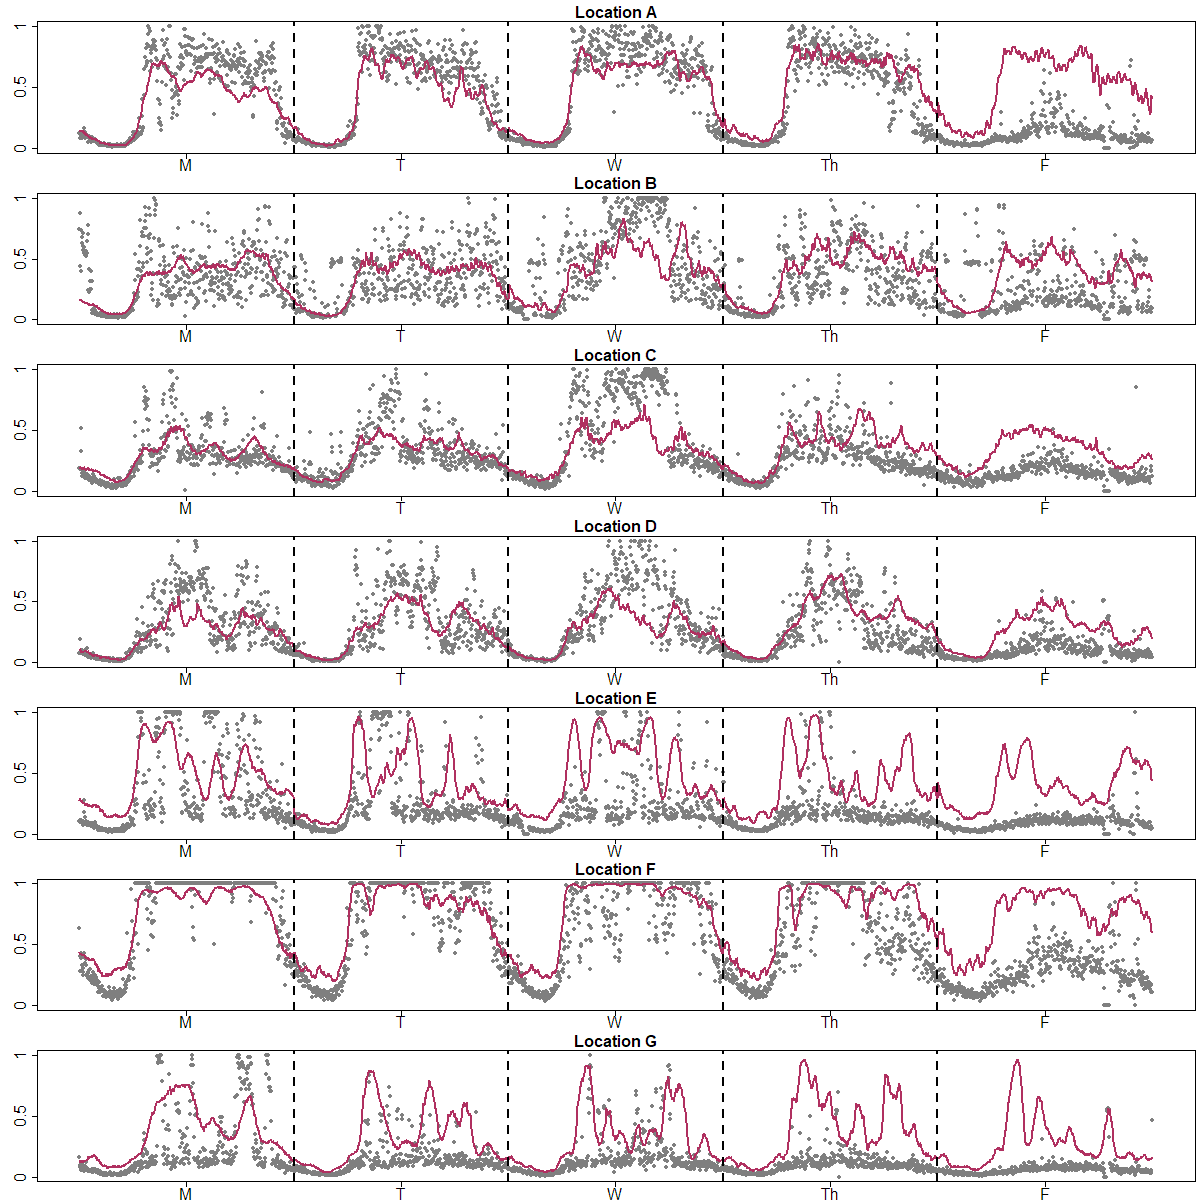
\includegraphics[width=\textwidth]{SEASESTPlots}
\label{fig:SEASESTPlots}
\end{figure}

\begin{figure}[htbp]
\caption{Forecasts Based on SEASt Models}
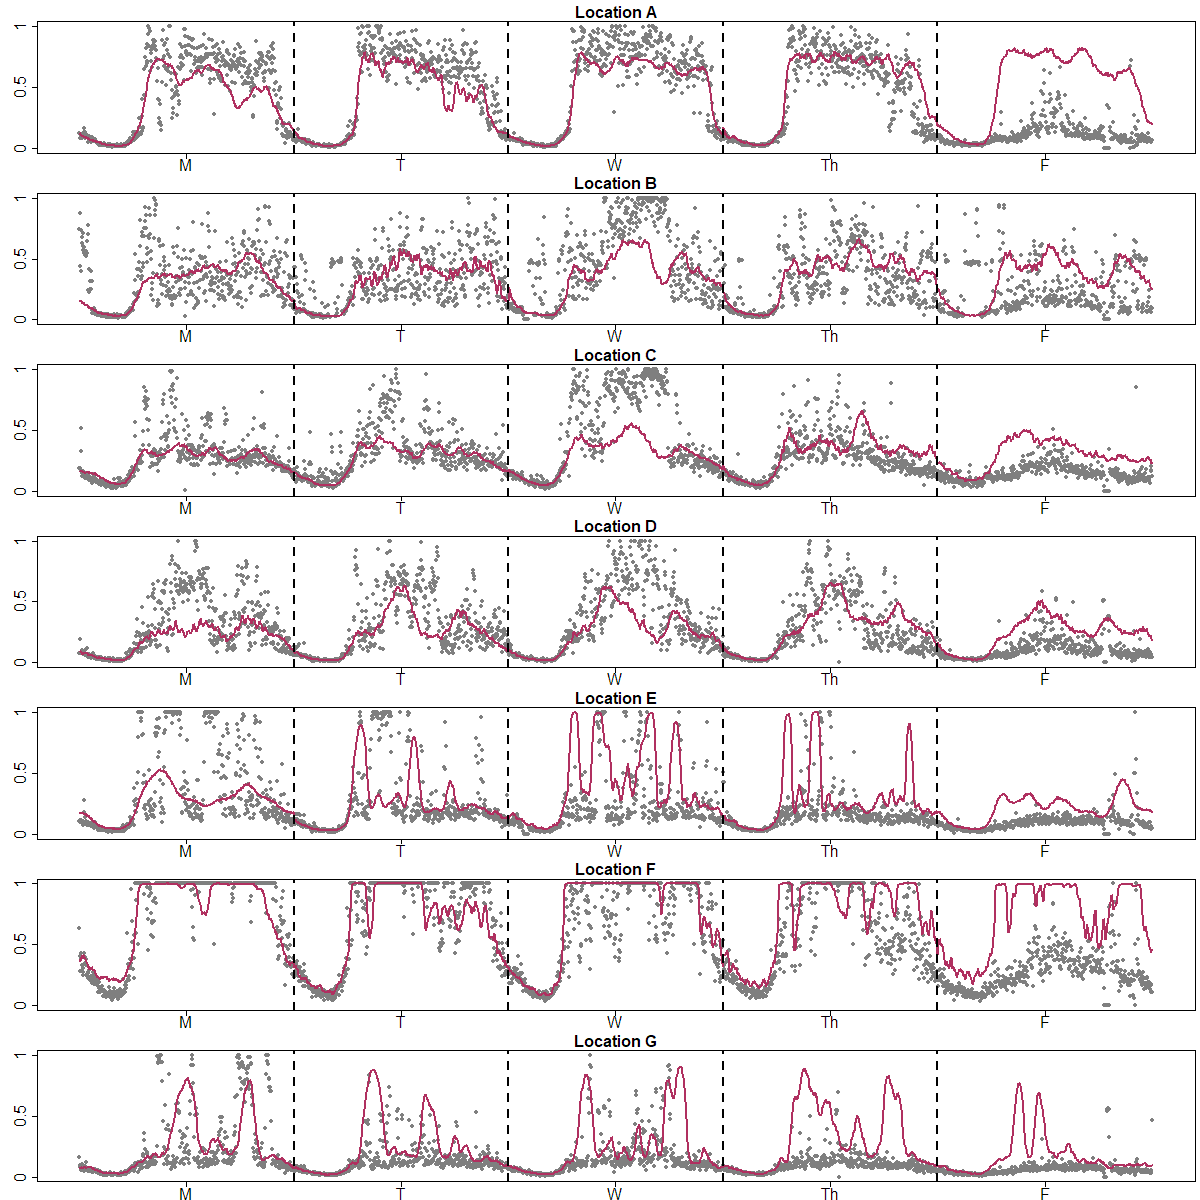
\includegraphics[width=\textwidth]{SEASESTtPlots}
\label{fig:SEASESTtPlots}
\end{figure}

On the original $[0,1]$-interval, we evaluate traffic occupancy forecasts over the final week of April using a rolling-window and without re-estimation. For each $(L,D,h)$-specific TAR and TARt model, we have $T_h=480-P-h+1$ time points requiring forecasts. Forecasts over this period are evaluated using the mean absolute scaled forecast error (MASFE) metric from \cite{Hyndman2006}. The formulation of MASE is found in Equation \ref{eq:trafficmase} where $\textrm{MAE}_{RW}(h)$ represents the mean absolute error from a $h$-specific naive random walk model over the fitting period. 
\begin{equation}
\label{eq:trafficmase}
  MASFE(h)=\frac{1}{T_h}\sum\limits_{t=P+h}^{480}\left|\frac{O_{L,t}-\widehat{O}_{L,t}}{\textrm{MAE}_{RW}(h)}\right|
\end{equation}

\begin{table}[htbp]
\scriptsize
\centering
\caption{1-Step Ahead MASE Forecast Comparison}
\begin{tabular}{c|rccccccc}
  \hline
  & & \multicolumn{7}{c}{Location}\\
  \cline{5-7}
Day & Model & A & B & C & D & E & F & G \\ 
  \hline
  \multirow{4}{*}{M} & TAR & 1.02 & 1.10 & 0.88 & 1.07 & 1.87 & 0.81 & 1.48 \\ 
  & TARt & 0.93 & 1.09 & 0.85 & 1.04 & 1.49 & 0.56 & 1.24 \\ 
  & SEAS & 1.80 & 1.47 & 1.15 & 1.43 & 4.02 & 1.57 & 3.66 \\ 
  & SEASt & 1.73 & 1.41 & 1.04 & 1.65 & 3.47 & 1.20 & 2.42 \\ 
  \hline
  \multirow{4}{*}{T}  & TAR & 0.90 & 1.05 & 1.04 & 0.98 & 1.36 & 1.03 & 1.95 \\ 
   & TARt & 0.89 & 1.05 & 0.96 & 0.95 & 0.98 & 0.77 & 1.30 \\ 
  & SEAS & 1.35 & 1.36 & 1.22 & 1.46 & 3.36 & 1.65 & 3.29 \\ 
   & SEASt & 1.33 & 1.32 & 1.20 & 1.50 & 2.47 & 1.46 & 2.03 \\ 
  \hline
   \multirow{4}{*}{W} & TAR & 1.04 & 1.11 & 0.91 & 0.97 & 2.27 & 1.86 & 1.55 \\ 
   & TARt & 0.99 & 1.14 & 1.01 & 0.99 & 1.30 & 1.75 & 1.38 \\ 
   & SEAS & 1.39 & 2.01 & 2.18 & 1.61 & 4.65 & 2.90 & 2.80 \\ 
   & SEASt & 1.17 & 1.96 & 2.35 & 1.63 & 3.49 & 2.34 & 2.16 \\ 
  \hline
 \multirow{4}{*}{Th} & TAR & 0.93 & 0.89 & 0.82 & 0.92 & 1.48 & 1.52 & 1.83 \\ 
   & TARt & 0.89 & 0.93 & 0.94 & 1.01 & 2.19 & 1.64 & 2.15 \\ 
   & SEAS & 1.44 & 1.43 & 1.51 & 1.42 & 3.98 & 2.74 & 4.07 \\ 
   & SEASt & 1.23 & 1.23 & 1.23 & 1.30 & 2.40 & 2.52 & 3.10 \\ 
  \hline
  \multirow{4}{*}{F} & TAR & 1.80 & 1.08 & 1.01 & 0.85 & 1.45 & 2.40 & 1.16 \\ 
   & TARt & 1.13 & 0.92 & 0.55 & 0.78 & 0.47 & 2.70 & 1.07 \\ 
   & SEAS & 4.77 & 2.23 & 1.98 & 1.83 & 4.37 & 6.24 & 3.78 \\ 
   & SEASt & 4.68 & 2.09 & 1.63 & 1.62 & 1.82 & 6.23 & 2.17 \\ 
   \hline
\end{tabular}
\label{ref:trafficmase1}
\end{table}

\begin{figure}[htbp]
\caption{1-Step Ahead Density Forecasts for TAR Models}
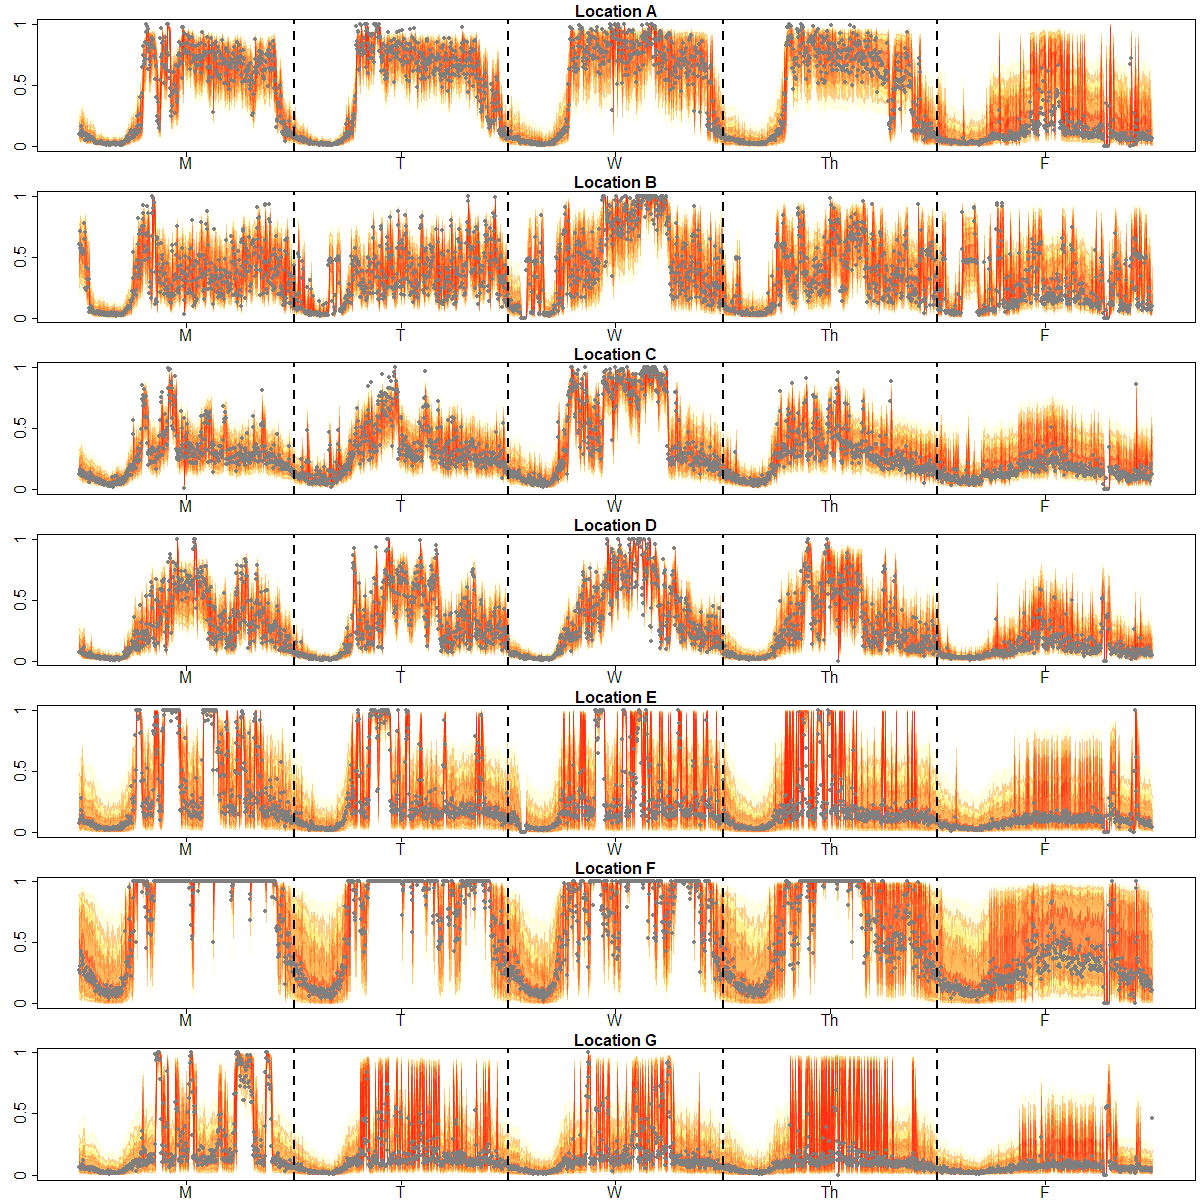
\includegraphics[width=\textwidth]{DENS1Plots}
\label{fig:DENS1Plots}
\end{figure}

\begin{figure}[htbp]
\caption{1-Step Ahead Density Forecasts for TARt Models}
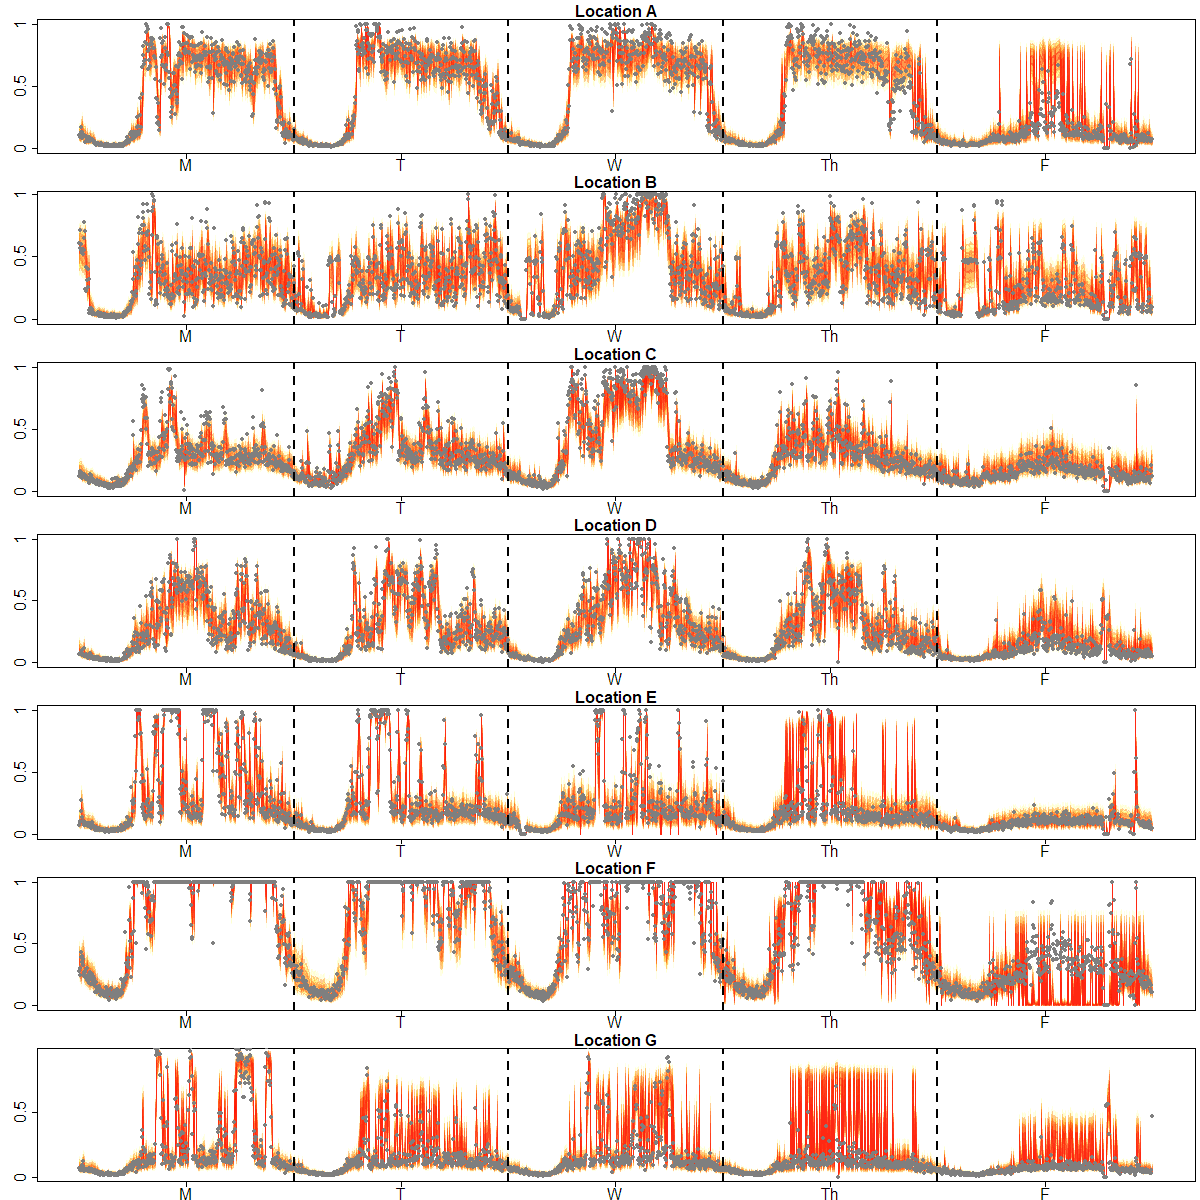
\includegraphics[width=\textwidth]{DENS1tPlots}
\label{fig:DENS1tPlots}
\end{figure}

\begin{table}[htbp]
\scriptsize
\centering
\caption{3-Step Ahead MASE Forecast Comparison}
\begin{tabular}{c|rccccccc}
  \hline
    & & \multicolumn{7}{c}{Location}\\
  \cline{5-7}
Day & Model & A & B & C & D & E & F & G \\ 
  \hline
  \multirow{4}{*}{M} & TAR & 0.94 & 1.06 & 0.88 & 1.13 & 1.85 & 0.88 & 1.50 \\ 
   & TARt & 0.89 & 1.03 & 0.80 & 1.13 & 1.52 & 0.59 & 1.26 \\ 
   & SEAS & 1.36 & 1.17 & 0.93 & 1.14 & 2.91 & 1.19 & 2.57 \\ 
   & SEASt & 1.31 & 1.12 & 0.84 & 1.30 & 2.51 & 0.91 & 1.70 \\ 
   \hline
  \multirow{4}{*}{T} & TAR & 0.87 & 1.04 & 0.96 & 1.03 & 1.46 & 1.15 & 1.21 \\ 
   & TARt & 0.79 & 1.02 & 0.92 & 0.97 & 1.00 & 0.86 & 0.96 \\ 
   & SEAS & 1.04 & 1.06 & 0.91 & 1.10 & 2.24 & 1.22 & 2.15 \\ 
   & SEASt & 1.02 & 1.03 & 0.89 & 1.13 & 1.65 & 1.08 & 1.32 \\
   \hline 
  \multirow{4}{*}{W} & TAR & 1.09 & 1.15 & 1.10 & 0.99 & 1.75 & 2.00 & 1.26 \\ 
   & TARt & 0.97 & 1.11 & 1.13 & 0.98 & 1.25 & 1.91 & 0.91 \\ 
   & SEAS & 1.15 & 1.61 & 1.69 & 1.21 & 2.94 & 2.24 & 1.71 \\ 
   & SEASt & 0.97 & 1.58 & 1.82 & 1.23 & 2.21 & 1.80 & 1.32 \\ 
   \hline
 \multirow{4}{*}{Th}  & TAR & 0.90 & 0.96 & 0.82 & 0.93 & 1.88 & 1.47 & 1.14 \\ 
   & TARt & 0.84 & 0.91 & 0.71 & 0.86 & 0.73 & 1.20 & 1.04 \\ 
   & SEAS & 1.15 & 1.09 & 1.14 & 1.03 & 2.69 & 1.96 & 2.68 \\ 
   & SEASt & 0.99 & 0.94 & 0.92 & 0.94 & 1.62 & 1.80 & 2.04 \\ 
  \hline
  \multirow{4}{*}{F} & TAR & 3.04 & 1.09 & 1.00 & 0.66 & 1.14 & 2.47 & 0.92 \\ 
   & TARt & 1.50 & 1.00 & 0.70 & 0.51 & 0.35 & 2.05 & 0.75 \\ 
   & SEAS & 3.53 & 1.57 & 1.42 & 1.33 & 3.12 & 4.35 & 2.42 \\ 
   & SEASt & 3.47 & 1.47 & 1.17 & 1.18 & 1.30 & 4.34 & 1.39 \\ 
   \hline
\end{tabular}
\label{ref:trafficmase3}
\end{table}

\begin{figure}[htbp]
\caption{3-Step Ahead Density Forecasts for TAR Models}
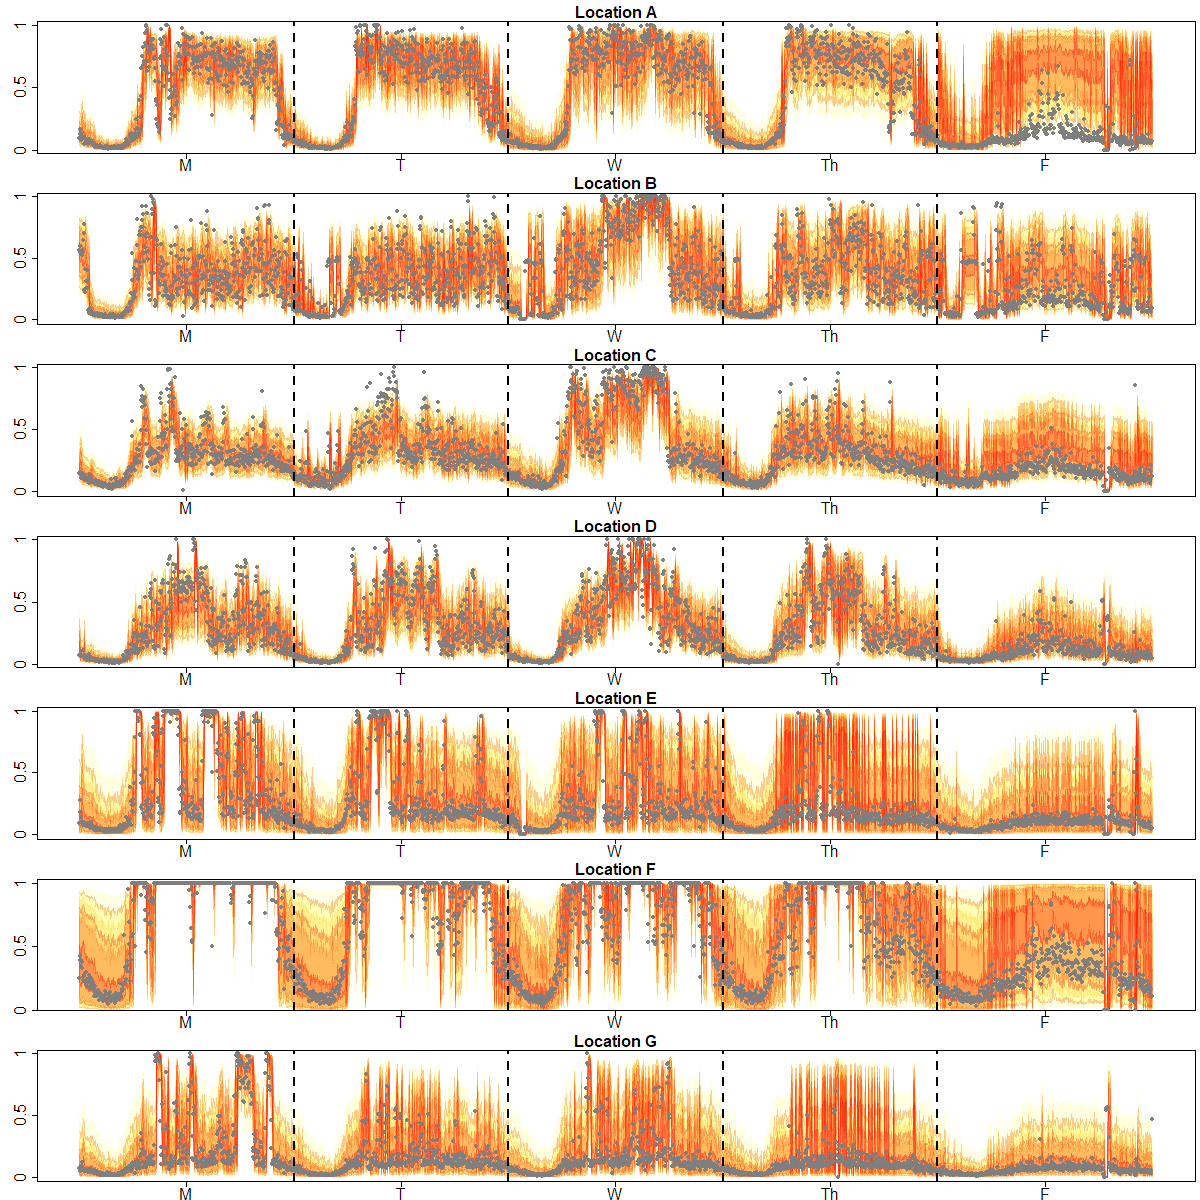
\includegraphics[width=\textwidth]{DENS3Plots}
\label{fig:DENS3Plots}
\end{figure}

\begin{figure}[htbp]
\caption{3-Step Ahead Density Forecasts for TARt Models}
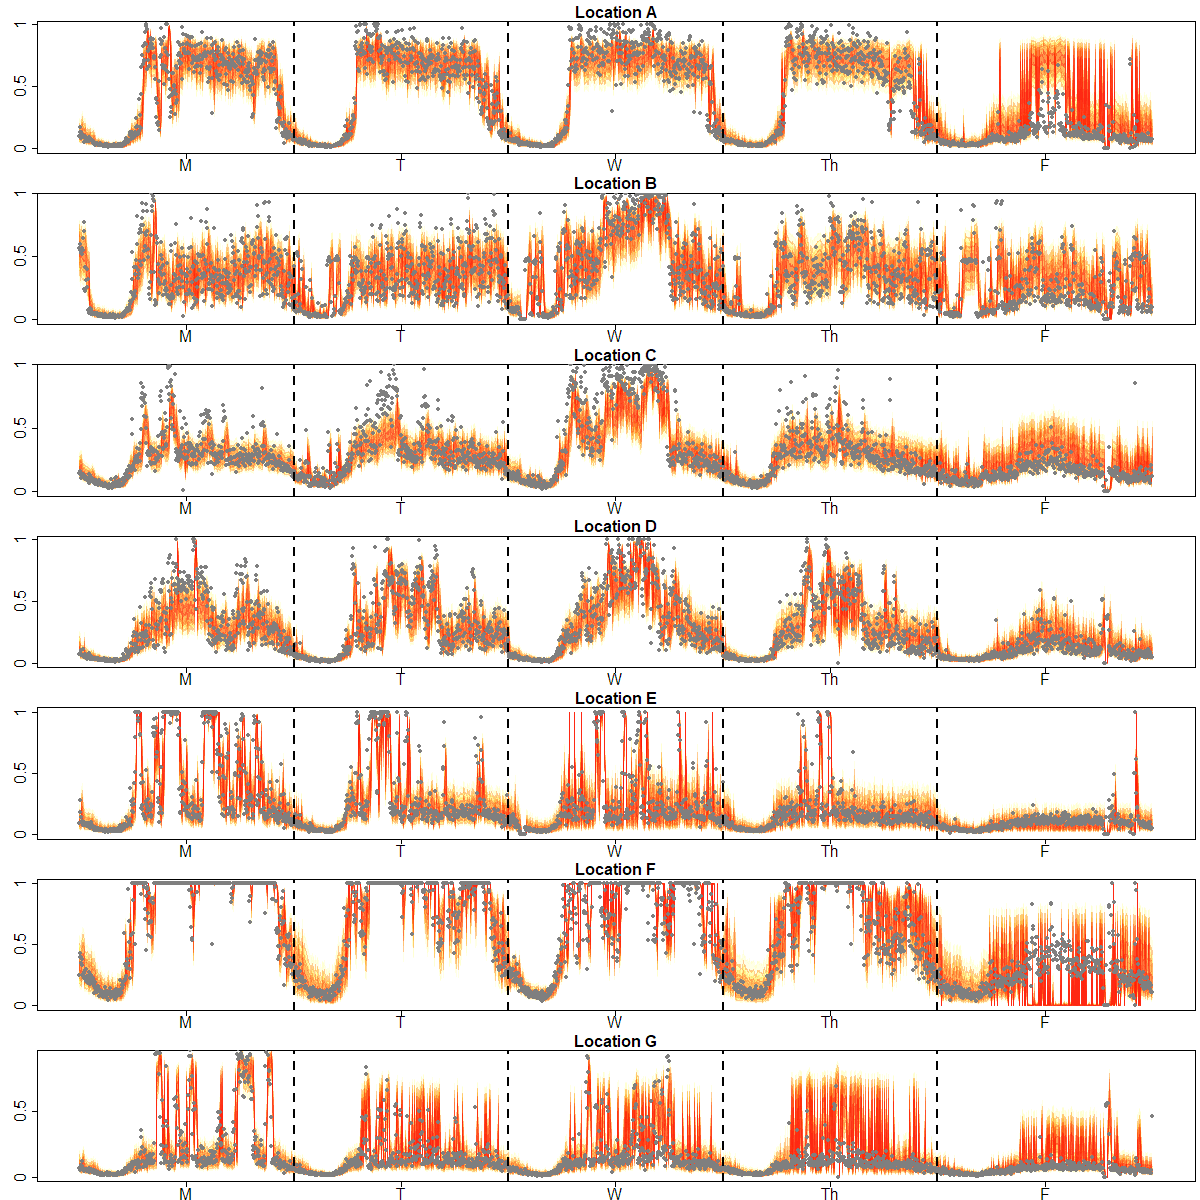
\includegraphics[width=\textwidth]{DENS3tPlots}
\label{fig:DENS3tPlots}
\end{figure}

\begin{table}[htbp]
\footnotesize
\centering
\caption{5-Step Ahead MASE Forecast Comparison}
\begin{tabular}{c|rccccccc}
  \hline
    & & \multicolumn{7}{c}{Location}\\
  \cline{5-7}
Day & Model & A & B & C & D & E & F & G \\ 
  \hline
  \multirow{4}{*}{M} & TAR & 0.94 & 0.99 & 0.89 & 1.12 & 1.97 & 0.86 & 1.68 \\ 
   & TARt & 0.92 & 0.95 & 0.81 & 1.15 & 1.58 & 0.58 & 1.22 \\ 
   & SEAS & 1.24 & 1.06 & 0.88 & 1.06 & 2.46 & 1.08 & 2.17 \\ 
   & SEASt & 1.19 & 1.02 & 0.80 & 1.22 & 2.12 & 0.83 & 1.43 \\ 
  \hline
  \multirow{4}{*}{T}  & TAR & 0.81 & 1.05 & 0.95 & 1.00 & 1.47 & 1.13 & 1.15 \\ 
   & TARt & 0.80 & 1.03 & 0.91 & 0.99 & 0.94 & 0.88 & 0.74 \\ 
   & SEAS & 0.95 & 0.95 & 0.85 & 0.99 & 1.85 & 1.07 & 1.77 \\ 
   & SEASt & 0.93 & 0.93 & 0.84 & 1.02 & 1.36 & 0.95 & 1.09 \\ 
  \hline
  \multirow{4}{*}{W}  & TAR & 1.02 & 1.12 & 1.04 & 0.99 & 1.67 & 1.94 & 1.26 \\ 
   & TARt & 0.90 & 1.12 & 0.96 & 0.98 & 1.43 & 1.81 & 0.86 \\ 
   & SEAS & 1.01 & 1.44 & 1.56 & 1.12 & 2.30 & 1.95 & 1.44 \\ 
   & SEASt & 0.85 & 1.40 & 1.68 & 1.14 & 1.73 & 1.57 & 1.11 \\ 
  \hline
  \multirow{4}{*}{Th}  & TAR & 0.84 & 0.98 & 0.82 & 0.87 & 1.51 & 1.48 & 1.22 \\ 
   & TARt & 0.78 & 0.91 & 0.68 & 0.80 & 0.69 & 1.08 & 0.95 \\ 
   & SEAS & 1.05 & 1.03 & 1.07 & 0.94 & 2.13 & 1.73 & 2.24 \\ 
   & SEASt & 0.90 & 0.89 & 0.87 & 0.86 & 1.28 & 1.59 & 1.71 \\ 
  \hline
  \multirow{4}{*}{F}  & TAR & 2.85 & 1.20 & 0.88 & 0.70 & 1.26 & 2.52 & 1.00 \\ 
   & TARt & 1.73 & 1.07 & 0.52 & 0.57 & 0.59 & 1.30 & 0.43 \\ 
   & SEAS & 3.07 & 1.48 & 1.33 & 1.19 & 2.59 & 3.82 & 2.01 \\ 
   & SEASt & 3.01 & 1.38 & 1.09 & 1.05 & 1.08 & 3.81 & 1.16 \\ 
   \hline
\end{tabular}
\label{ref:trafficmase5}
\end{table}

\begin{figure}[htbp]
\caption{5-Step Ahead Density Forecasts for TAR Models}
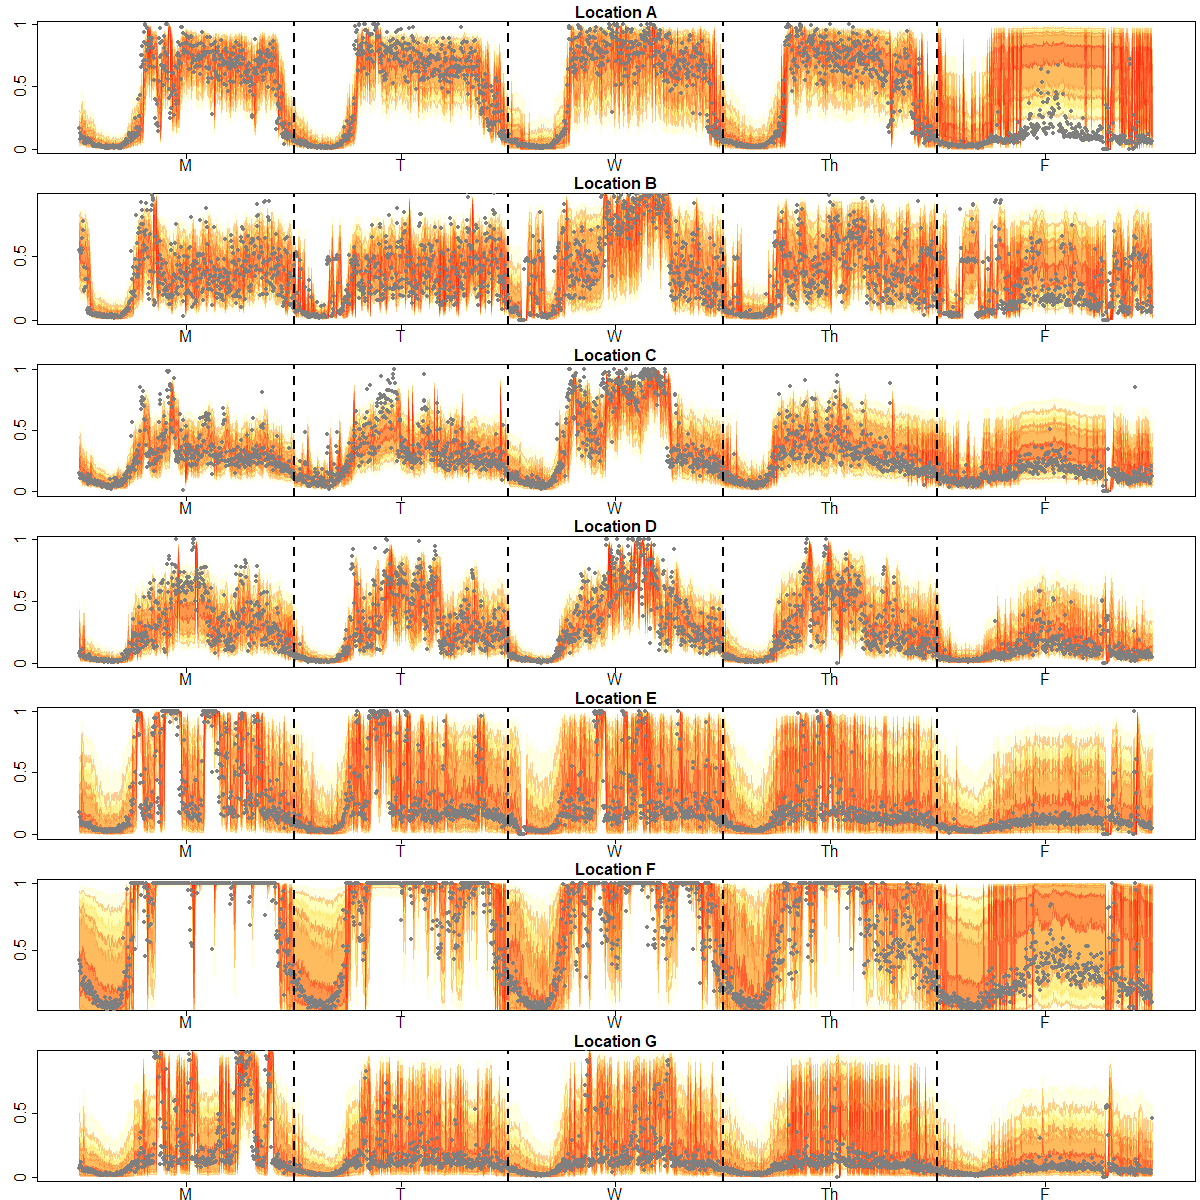
\includegraphics[width=\textwidth]{DENS5Plots}
\label{fig:DENS3Plots}
\end{figure}

\begin{figure}[htbp]
\caption{5-Step Ahead Density Forecasts for TARt Models}
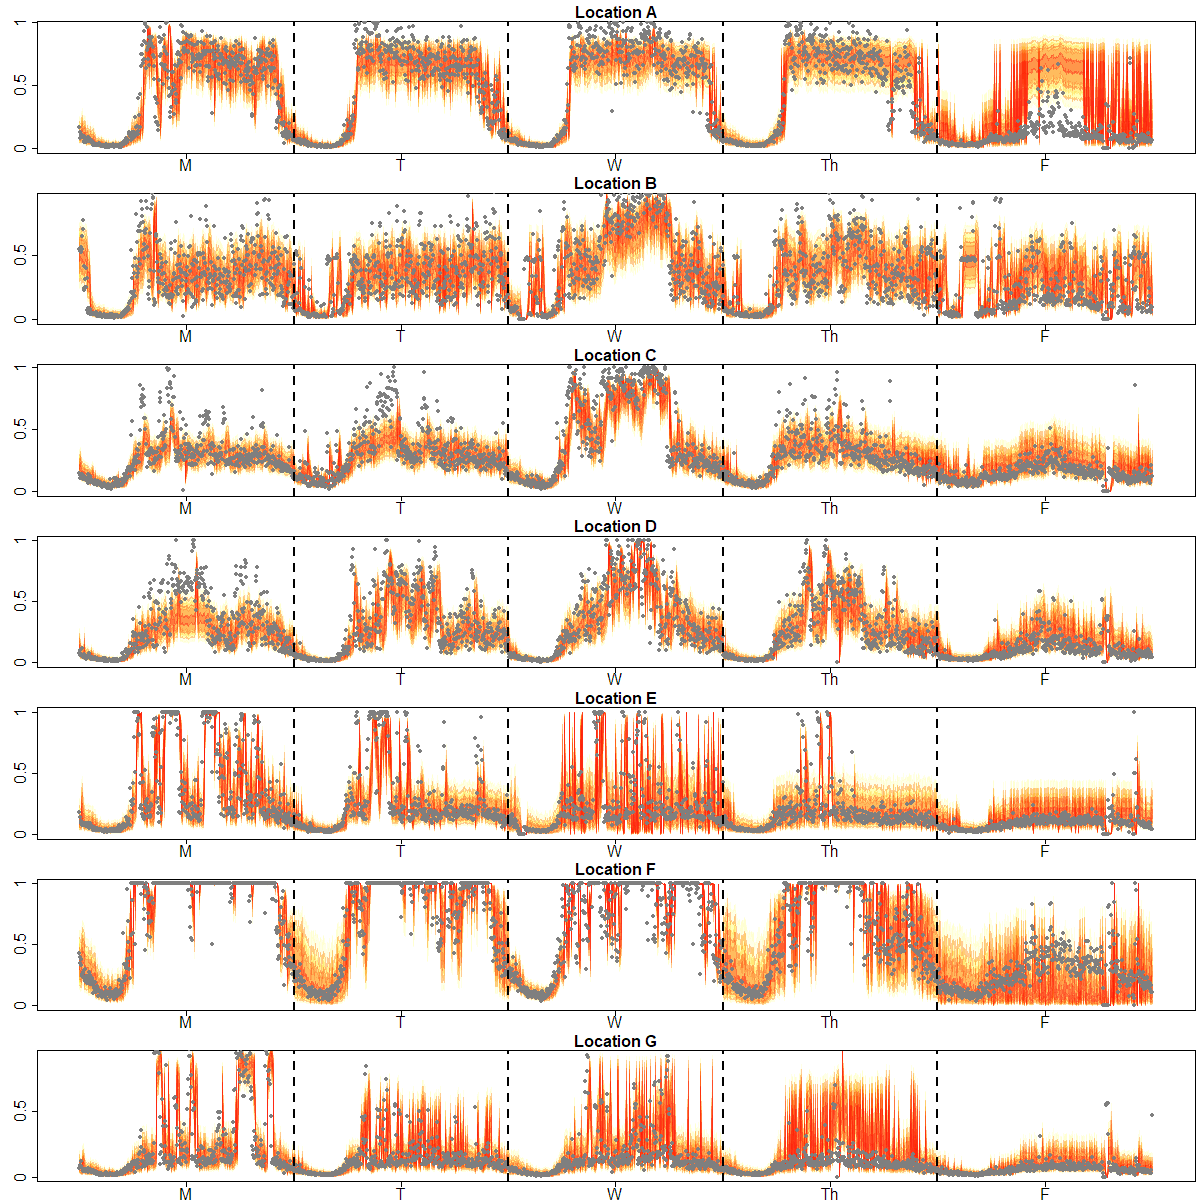
\includegraphics[width=\textwidth]{DENS5tPlots}
\label{fig:DENS3tPlots}
\end{figure}

















\section{Conclusion}
















\bigskip
\bigskip
\bigskip
\bigskip
\bigskip


\subsection{Kullback-Leibler Discrimination}
The joint posterior distribution $f(\bm{\theta}_{\mathcal{M}_R}|\mathcal{M}_R,\mathcal{I})$ obtained through BHS priors is  a good starting point. Although BHS priors separately invoked on $\bm{\alpha}$ and $\bm{\beta}$ lead to regime-specific sparse estimation, it is unlikely posterior means $E[\bm{\alpha}|\mathcal{M}_R,\mathcal{I}]$ and $E[\bm{\beta}|\mathcal{M}_R,\mathcal{I}]$ contain true $0$ values.   Assuming the data follows some TAR process, the model space containing all submodels of $\mathcal{M}_R$ contains $2^{2(P+1)}$ different alternatives. Naively exploring this model space to find the best reduced model $\mathcal{M}^*_R$ is an inefficient approach.

The Kullback-Leibler (KL) divergence is an asymmetric measure of distance between two probability distributions\citep{Kullback1951}. \cite{burnham2003} provides a nice discussion connecting KL divergence to subset model selection based on Aikaike information criteria (AIC). \cite{Goutis1998} and \cite{Dupuis2003} use KL divergence to compare a proposed submodel to a larger reference model based on conditional likelhoods. If minor discrepancy is detected between the reference model and a particular submodel, the simpler submodel can be considered. The proposed method derives a posterior distribution for a submodel through projection from the information in the sampled posterior distribution for the larger reference model. \cite{Piironen2017} provided analytical solutions to obtain the projected parameters and evaluate the resulting KL divergence for Gaussian linear models. For $\mathcal{M}_R$, we treat $\mathcal{M}_{LR}$ and $\mathcal{M}_{HR}$ as reference models for the corresponding regimes. Both $\mathcal{M}_{LR}$ and $\mathcal{M}_{HR}$ are conditionally linear Gaussian models; therefore we extend the methods of \cite{Piironen2017} to the general TAR($P$). 

Let $\bm{Y_{t-1}}$ be the $T\times(P+1)$ matrix where the $k$th row is the vector of lagged information $\bm{y_{k-1}}'=[1,y_{k-1},y_{k-2},\cdots,y_{k-P}]$. We define $\bm{\theta}^{(s)}$ as the $s$th posterior draw from $f(\bm{\theta}_{\mathcal{M}_R}|\mathcal{M}_R,\mathcal{I})$ partitioned by $[\bm{\alpha}^{(s)},\sigma_\alpha^{(s)},\bm{\beta}^{(s)},\sigma_\beta^{(s)},\delta^{(s)}]$. Now, consider an arbitrary submodel $\mathcal{M}^\perp_{R}$ characterized by  $\mathcal{M}^\perp_{LR}$ and $\mathcal{M}^\perp_{HR}$. Similarly, define the $s$th draw from the posterior $f(\bm{\theta}_{\mathcal{M}^\perp_R}|\mathcal{M}^\perp_R,\mathcal{I})$  as $\bm{\theta}^{\perp(s)}=[\bm{\alpha}^{\perp(s)},\sigma_\alpha^{\perp(s)},\bm{\beta}^{\perp(s)},\sigma_\beta^{\perp(s)},\delta^{(s)}]$.  
 
Given $\bm{\theta}^{(s)}$, we start by splitting model matrix $\bm{Y_{t-1}}$ into two smaller matrices $\bm{Y_{LR,t-1}}$ and $\bm{Y_{HR,t-1}}$ based on the sampled threshold $\delta^{(s)}$. $\bm{Y_{LR,t-1}}$ contains the rows of $\bm{Y_{t-1}}$ corresponding to the times whenever $z_t<\delta$, and $\bm{Y_{HR,t-1}}$ contains the rows of  $\bm{Y_{t-1}}$ not contained in $\bm{Y_{LR,t-1}}$. Furthermore, $\bm{Y^{\perp}_{LR,t-1}}$ and $\bm{Y^{\perp}_{HR,t-1}}$ contain the columns of $\bm{Y_{LR,t-1}}$ and $\bm{Y_{HR,t-1}}$ reflective of the proposed regime-specific submodels $\mathcal{M}^\perp_{LR}$ and $\mathcal{M}^\perp_{HR}$, respectively. For each $s \in \{1,2,\cdots,S\}$, we sample $\bm{\theta}^{\perp(s)}$ from the  projected posterior $f(\bm{\theta}_{\mathcal{M}^\perp_R}|\mathcal{M}^\perp_R,\mathcal{I})$ by applying Equation \ref{eq:proj} to the original $\bm{\theta}^{(s)}$ drawn under BHS priors.
\begin{equation}
\label{eq:proj}
\begin{split}
\bm{\alpha}^{\perp(s)}&=(\bm{Y^{\perp'}_{LR,t-1}}\bm{Y^{\perp}_{LR,t-1}})^{-1} \bm{Y^{\perp'}_{LR,t-1}}     \bm{Y_{LR,t-1}}\bm{\alpha}^{(s)}\\
\sigma_\alpha^{\perp(s)}&=\sqrt{(\sigma_\alpha^{(s)})^2+\frac{( \bm{Y_{LR,t-1}}\bm{\alpha}^{(s)}-\bm{Y^\perp_{LR,t-1}}\bm{\alpha}^{\perp(s)})'( \bm{Y_{LR,t-1}}\bm{\alpha}^{(s)}-\bm{Y^\perp_{LR,t-1}}\bm{\alpha}^{\perp(s)})}{T}                                  }\\
\bm{\beta}^{\perp(s)}&=(\bm{Y^{\perp'}_{HR,t-1}}\bm{Y^{\perp}_{HR,t-1}})^{-1} \bm{Y^{\perp'}_{HR,t-1}} \bm{Y_{HR,t-1}}\bm{\beta}^{(s)}\\
\sigma_\beta^{\perp(s)}&=\sqrt{(\sigma_\beta^{(s)})^2+\frac{( \bm{Y_{HR,t-1}}\bm{\beta}^{(s)}-\bm{Y^\perp_{HR,t-1}}\bm{\beta}^{\perp(s)})'( \bm{Y_{HR,t-1}}\bm{\beta}^{(s)}-\bm{Y^\perp_{HR,t-1}}\bm{\beta}^{\perp(s)})}{T}                                   }
\end{split}
\end{equation}

For each posterior draw from $f(\bm{\theta}_{\mathcal{M}_R}|\mathcal{M}_{R},\mathcal{I})$, we measure the corresponding regime-specific KL divergences $d_{LR}$ and $d_{HR}$ using Equation \ref{eq:klds}.
\begin{equation}
\label{eq:klds}
\begin{split}
d^{(s)}_{LR}(\bm{\alpha}^{(s)},\sigma^{(s)}_\alpha)&=\log\bigg(\frac{\sigma^{\perp(s)}_\alpha}{\sigma^{(s)}_\alpha}\bigg)^2\\
d^{(s)}_{HR}(\bm{\beta}^{(s)},\sigma^{(s)}_\beta)&=\log\bigg(\frac{\sigma^{\perp(s)}_\beta}{\sigma^{(s)}_\beta}\bigg)
\end{split}
\end{equation}

Finally, measures $D(\mathcal{M}_{LR}||\mathcal{M}^\perp_{LR})$ and $D(\mathcal{M}_{HR}||\mathcal{M}^\perp_{HR})$ expressed in Equation \ref{eq:disc} determine the discrepancy between regime-specific full models to proposed reduced versions. 
\begin{equation}
\label{eq:disc}
\begin{split}
D(\mathcal{M}_{LR}||\mathcal{M}^\perp_{LR})&=\frac{1}{S}\sum\limits^S_{s=1} d^{(s)}_{LR}(\bm{\alpha}^{(s)},\sigma^{(s)}_\alpha)    \\
D(\mathcal{M}_{HR}||\mathcal{M}^\perp_{HR})&=\frac{1}{S}\sum\limits^S_{s=1} d^{(s)}_{HR}(\bm{\beta}^{(s)},\sigma^{(s)}_\beta)     \\
\end{split}
\end{equation}

Using these concepts, we avoid surveying the entire  $2^{2(P+1)}$ model space by employing a forward stepwise selection algorithm to identify the best regime-specific submodel at every possible level of flexibility bounded by predetermined $P$. The simplest models considered are the intercept-only models denoted $\mathcal{M}^0_{LR}$ and $\mathcal{M}^0_{HR}$. The initial discrepancies  $D(\mathcal{M}_{LR}||\mathcal{M}^0_{LR})$ and $D(\mathcal{M}_{HR}||\mathcal{M}^0_{HR})$ represent the maximum divergence between the full models and all possible submodels. 

For each level of flexibility $p \in \{1,2,\cdots,P\}$, we find the best regime-specific submodels $\mathcal{M}^p_{LR}$ and $\mathcal{M}^p_{HR}$. Starting with $p=1$, we consider all two dimensional submodels including the intercept and one lagged term. $\mathcal{M}^1_{LR}$ and $\mathcal{M}^1_{HR}$ are chosen based on minimized discrepancy when compared to the full model. Then for $p=2$, all three dimensional regime-specific submodels nesting $\mathcal{M}^1_{LR}$ and $\mathcal{M}^1_{HR}$ are compared to the corresponding full models to find $\mathcal{M}^2_{LR}$ and $\mathcal{M}^2_{HR}$. Continuing this process results in $P+1$ considerations for $\mathcal{M}_{LR}$ and $P+1$ considerations for $\mathcal{M}_{HR}$. 

\subsection{Final Model Selection}
The final reduced models $\mathcal{M}^*_{LR}$ and $\mathcal{M}^*_{HR}$ are chosen from the $2P+2$ options identified through the forward stepwise algorithm. \cite{Dupuis2003} utilized the additive properties of KL divergence for nested models to choose the best model based on relative explanatory power defined in Equation \ref{eq:rep}. As $p$ goes from $0$ to $P$, RelE strictly increases from 0 to 1. As noted by \cite{Dupuis2003} and \cite{Piironen2017}, $\mathcal{M}^*_{LR}$ and $\mathcal{M}^*_{HR}$ can be the smallest submodels that achieve a $RelE > E^*$, where $E^*$ is a predetermined threshold. It is recommended $E^*$ be large i.e. $>90\%$.
\begin{equation}
\label{eq:rep}
\begin{split}
RelE(\mathcal{M}^p)&=1-\frac{D(\mathcal{M}||\mathcal{M}^p)}{D(\mathcal{M}||\mathcal{M}^0)}\\
\end{split}
\end{equation}

\cite{Piironen2015,Piironen2017} favors final selection based on out-of-sample prediction. Regarding time series models, this implies forecasting performance. We choose the final regime-specific reduced models $\mathcal{M}^*_{LR}$ and $\mathcal{M}^*_{HR}$ based on the minimization of  regime-specific root mean squared forecast error (RMSFE) over a time period intentionally left out. The formula for RMSFE is stated in \ref{eq:rmsfe1}.
\begin{equation}
 	\label{eq:rmsfe1}
  RMSFE(\mathcal{M}^p)=\sqrt{\frac{1}{T}\sum (y_t-\hat{y}_t)^2}
\end{equation}










%%%%%%%%%%%%%%%%%%%%%%%%%%%%%%%%%%%%%%%%%%%%%%%%%%%%%%%%%%%%%%%%%%%%%%%%
\section{Forecasting Evaluation}
Threshold autoregressive models for traffic occupancy are obvious, considering the structural differences between free flow and congested states. Although practice invites these considerations, it is not necessary that TAR models achieve optimal forecasting accuracy over linear models. Even under nonlinear simulated data, \cite{Davies1988} and \cite{Pemberton1989} illustrated that linear models can occasionally achieve equivalent or better forecasting accuracy than nonlinear competitors \citep{Guo1997,Stock1998a,Dacco1999}.

Given arbitrary full model  $\mathcal{M}$, the methods in Section \ref{sec:bayesest} lead us to final submodel $\mathcal{M}^*$. Final selection of $\mathcal{M}^*$ was indicative of optimal forecasting performance at a specific horizon $h$. By design, optimal forecasts and credible regions for $y_{B,t+h}$ are based on the simulated predictive posterior distribution $f_Y(y_{B,t+h}|\mathcal{I})$ defined on $\mathbb{R}$. The inverse logit function $\phi^{-1}(x):\mathbb{R}\to (0,1)$ where $\phi^{-1}(x)=\exp(x)/[1+\exp(x)]$ provides a path from $f_Y(y_{B,t+h}|\mathcal{I})$ to $f_O(o_{B,t+h}|\mathcal{I})$. Let $\widehat{Y}_{B,t+h}=E[Y_{B,t+h}|\mathcal{I}]$. Because $\phi(x)$ is a nonlinear transformation, $\widehat{O}_{B,t+h}=E[O_{B,t+h}|\mathcal{I}] \neq \phi^{-1}(\widehat{Y}_{B,t+h})$. The natural bias and correction method introduced from nonlinear transformations (i.e. general log function) is discussed in \cite{Metcalfe2009}. For $s \in \{1,2,\cdots, S\}$, we simulate $f_O(o_{B,t+h}|\mathcal{I})$ using posterior draws $y^{(s)}_{B,t+h}$ from $f_Y(y_{B,t+h}|\mathcal{I})$. Figure \ref{fig:posttrans} graphically portrays this process.

\begin{figure}[!h]
\label{fig:posttrans}
\caption{Path to Obtain the Posterior Distribution $f_O(o_{B,t+h}|\mathcal{I})$ from the Posterior Distribution  $f_Y(y_{B,t+h}|\mathcal{I})$ Using Monte Carlo Draws}
\centering
\begin{tikzpicture}[line width=1pt,>=latex]
\sffamily
\node (a2) {$y^{(s)}_{B,t+h}$};

\node[right=5cm of a2] (b2) {$o^{(s)}_{B,t+h}$};

\node[shape=ellipse,draw,minimum size=2.5cm,fit={(a2)}] {};
\node[shape=ellipse,draw,minimum size=2.5cm,fit={(b2)}] {};

\node[below=1.25cm of a2,font=\Large\bfseries] {$f_Y(y_{B,t+h}|\mathcal{I})$};
\node[below=1.25cm of b2,font=\Large\bfseries] {$f_O(o_{B,t+h}|\mathcal{I})$};

\draw[->,black] (a2) -- node[label=above:$\phi^{-1}(x)$] {} (b2);
\end{tikzpicture}
\end{figure}



Define $\mathbb{M}=\{L_1(D,h), R_1(D,h), L_2(D,h), R_2(D,h)\}$ to be the set of all full models and $\mathbb{M}^*=\{L^*_1(D,h), R^*_1(D,h), L^*_2(D,h), R^*_2(D,h)\}$ to be the corresponding reduced models. Given day $D$ and horizon $h$, we use three forecast accuracy metrics to answer the following quesions about $\mathbb{M}$ and $\mathbb{M}^*$:    
\begin{itemize}
   \item How do the models compare to each other?
   \item How do the full models compare to the final models?
   \item How do the models compare to benchmark naive and seasonal models?
 \end{itemize}


\begin{equation}
\label{eq:srelmafe}
  SRelMAFE(h)=\frac{1}{n_h}\sum\limits_{t=h+1}^{480}\left|\frac{O_{B,t}-\widehat{O}_{B,t}}{\textrm{MAE}_{S}}\right|
\end{equation}



